\chapter{Boolean Algebra \& Logic Gates}

Boolean algebra is a branch of mathematics that deals with logical operations on binary variables.

\section{Rules and Theorems}

Associative, demorgan, blah blah

\section{Basic Logic Gates}

\subsection{AND}

\begin{figure}[h!]
	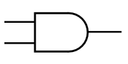
\includegraphics{./img/and-gate.png}
\end{figure}

\begin{tabular}{c c c}
	\hline
	\textbf{x} & \textbf{y} & \textbf{x \& y} \\ 
	\hline
	0 & 0 & 0 \\
	0 & 1 & 0 \\
	1 & 0 & 0 \\
	1 & 1 & 1 \\
	\hline 
\end{tabular} \\

\subsection{OR}

\begin{tabular}{c c c}
	\hline
	\textbf{x} & \textbf{y} & \textbf{x + y} \\ 
	\hline
	0 & 0 & 0 \\
	0 & 1 & 1 \\
	1 & 0 & 1 \\
	1 & 1 & 1 \\
	\hline 
\end{tabular} \\

\subsection{NOT}

\begin{tabular}{c c}
	\hline
	\textbf{x} & \textbf{¬x} \\ 
	\hline
	0 & 1  \\
	1 & 0  \\
	\hline 
\end{tabular} \\